\documentclass[11pt,a4paper]{article}
\usepackage[margin=0.95in]{geometry}
\usepackage{amsmath,amssymb,booktabs,graphicx,hyperref,enumitem,float,array}
\usepackage{fancyhdr}
\pagestyle{fancy}
\fancyhf{}
\lhead{AI651 Assignment 2}
\rhead{Fall 2026}
\cfoot{\thepage}
\setlength{\parskip}{0.35em}
\setlength{\parindent}{0pt}
\graphicspath{{Question2/results/}}

\title{Assignment 2 Report\\[0.2em]\large AI651 --- Deep Learning for Space, Time and Graphs}
\author{Roll number: 25280044}
\date{Fall 2026}

\begin{document}
\maketitle

\noindent
\textbf{Roll number:} 25280044\\
\textbf{GitHub (public):} \texttt{https://github.com/junaid074/DL4STG-PA2}

\vspace{0.25em}
\noindent
Q1: design only.\\
Q2 code: \texttt{Question2/}. Hardware: Apple M2 Max (PyTorch MPS).\\
Every learned-model entry is mean (seed 0, seed 1). Errors to three significant figures.

% ============================================================
\section{Question 1 --- River Forecasting Proposal}

\subsection{1. Architecture diagram}

\begin{verbatim}
 R1,R2 (hist) ----\
 T1 (hist) --------+--> 10-min align --> Enc_exog (causal CNN/GRU)
 Releases past+fut/
                          |
 S1..S4 levels (hist) --> Enc_T (per station)
                          |
              river line-graph  S1 -> S2 -> S3 -> S4
              (T1 joins on edge into S2; edge feat: dist, tau-hat)
                          |
                    K hops of message passing (ST stack)
                          |
              decode S1..S4 --> 6 steps (1 hour @ 10 min)
\end{verbatim}

Tensors (batch $B$ omitted): levels $Y\in\mathbb{R}^{5\times L}$ (S1--S4,T1); rain $R\in\mathbb{R}^{2\times L}$; releases $U\in\mathbb{R}^{L+H}$; latents $H\in\mathbb{R}^{4\times L\times d}$; forecast $\widehat Y\in\mathbb{R}^{4\times H}$ with $L=36$, $H=6$, $d\sim 64$.

\subsection{2. Assumptions}

\textbf{A1.} All series share a 10-minute clock after interpolation (normal for SCADA).\\
\textbf{A2.} Announced releases for the next hour are known at issuance (given).\\
\textbf{A3.} Travel time is a slow function of recent stage; we keep a distance prior $\hat\tau_{ij}\propto\mathrm{dist}_{ij}$ and let the net correct it.\\
\textbf{A4.} The unmonitored tributary is a residual inflow into S3 --- no fake gauge.\\
\textbf{A5.} Six hours of history ($L=36$) covers recent waves and release effects.\\
\textbf{A6.} Noise is roughly additive; Huber loss is enough (full flood PDF optional).

\subsection{3. Forecasting task and data specification}

Issuance every 10 min at $t_0$. History $[t_0-L\Delta t,t_0]$. Horizon $H=6$ (one hour). Outputs: S1--S4 only.

\begin{center}
\small
\begin{tabular}{llp{5.2cm}}
\toprule
Name & Shape & Coverage \\
\midrule
levels S1--S4,T1 & $B\times5\times L$ & past to $t_0$ \\
rain R1,R2 & $B\times2\times L$ & past \\
releases & $B\times(L+H)$ & past + announced future \\
static graph & edges, distances & fixed \\
output & $B\times4\times H$ & future S1--S4 \\
\bottomrule
\end{tabular}
\end{center}

At issuance: no future rain, no future levels; future releases yes. Late rain uses last value + missing bit.

\subsection{4. Model computations and design justification}

Per-station encode $z_i=\mathrm{Enc}_T(Y_i,e_i)$. One hop:
\[
\tilde z_i = z_i + \sum_{j\in\mathcal{N}_{\mathrm{in}}(i)}
\alpha_{ji}\,\psi(z_j,z_i,\mathrm{dist}_{ji},\hat\tau_{ji}).
\]
Stack $K\ge 3$ so S1 can reach S4. Head maps $(\tilde z_i,U_{\mathrm{future}})$ to $H$ steps. Loss: mean Huber on S1--S4 over the horizon.

Releases and upstream rain hit S1 first, then hop downstream. T1 enters the S1$\to$S2 edge. S3 never sees the unmonitored tributary directly --- only S2 plus a learned residual (A4). $\hat\tau$ is a prior, not a hard delay line.

\subsection{5. Operation and exceptional conditions}

\textbf{(i) Missing:} last value + mask; drop a dark station from the sum after 3 gaps but still decode it from neighbours.\\
\textbf{(ii) Delayed:} issue on the latest complete snapshot; late packets update the next cycle.\\
\textbf{(iii) Announced releases:} feed $U_{t_0+1:t_0+H}$ as known decoder inputs.\\
\textbf{(iv) Schedule vs actual:} mismatch shows up at S1 next step and propagates; optional 1-step residual on S1.\\
Runtime: four stations, $L=36$, $K\le4$ --- well under a second on CPU every 10 minutes.

\subsection{6. Uncertainty, limitations, and additional information}

Unmonitored tributary can bias S3/S4 after local storms --- request a cheap stage gauge. Changing travel times in flood --- request occasional discharge checks to retune $\hat\tau$. Rain beyond R1/R2 --- request radar QPE. Without those the service still runs; it just leans on recent downstream readings and is weaker on rare tributary-driven events.

% ============================================================
\section{Question 2 --- Motion or Memory?}

\subsection*{Table 1 --- checks}

All eight checks matched the handout exactly (max abs diffs 0; bright pixels $(7,10,43)$ and $(7,43,10)$; windows 1$\times$/2$\times$/3$\times$ as specified).

\subsection*{Figure 1 and Q2.1--Q2.2}

\begin{figure}[H]
\centering
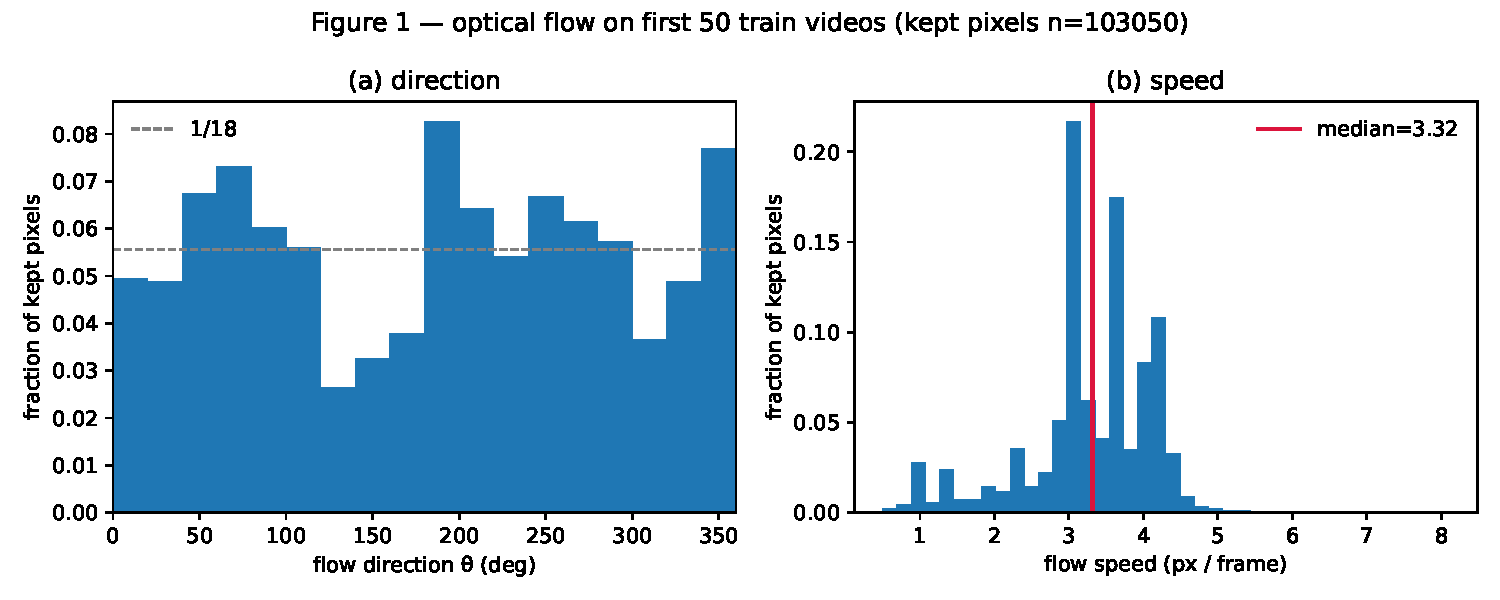
\includegraphics[width=0.95\textwidth]{figure1.pdf}
\caption{Figure 1 --- Farneback flow, first 50 training videos. Kept pixels $n=103050$; median speed $3.32$ px/frame.}
\end{figure}

\textbf{Q2.1.} The direction histogram is not a perfect flat $1/18$ line, but it has mass in many bins, so mirrored and $90^\circ$-rotated trajectories are already partly familiar --- flipping/rotating the rose roughly permutes bins that already have counts. Typical speed $\approx 3.3$ px/frame, so 2$\times\approx 6.6$ and 3$\times\approx 9.9$ px/frame. Overlap makes Farneback noisy, but with $>10^5$ kept pixels that should not flip the ``mostly familiar directions / median $\sim$3'' story.

\textbf{Q2.2.} Mirror and rotation keep the motion family but change digit appearance. Speed-up keeps appearance and changes how far digits jump. That splits appearance-tied failures from unfamiliar speeds from pure reach limits.

\subsection*{Model A, reach, Table 2, Figure 2}

\textbf{Q2.3.} Patch size 4 $\Rightarrow$ one folded cell $=4$ original pixels. Each $3\times 3$ moves 1 cell. Longest path in one step: input $\to$ ConvLSTM1 $\to$ ConvLSTM2 $\to$ head $=2$ cells $=8$ px/step. Reach$(A)=8$.

\begin{center}
\small
\begin{tabular}{lcccccc}
\toprule
Model & MSE$_1$ & MSE$_2$ & MSE$_3$ & MSE$_4$ & MSE$_5$ & $E(5)$ \\
\midrule
A & 0.0169 (0.0173, 0.0166) & 0.0202 (0.0207, 0.0198) & 0.0224 (0.0229, 0.0219) & 0.0241 (0.0247, 0.0236) & 0.0258 (0.0263, 0.0253) & 0.0219 (0.0224, 0.0214) \\
Blank & 0.0426 & 0.0426 & 0.0426 & 0.0425 & 0.0425 & 0.0426 \\
Copy-last & 0.0492 & 0.0604 & 0.0669 & 0.0708 & 0.0732 & 0.0641 \\
\bottomrule
\end{tabular}
\end{center}
\noindent
Table 2 --- test set. A has 480{,}784 parameters.

\begin{figure}[H]
\centering
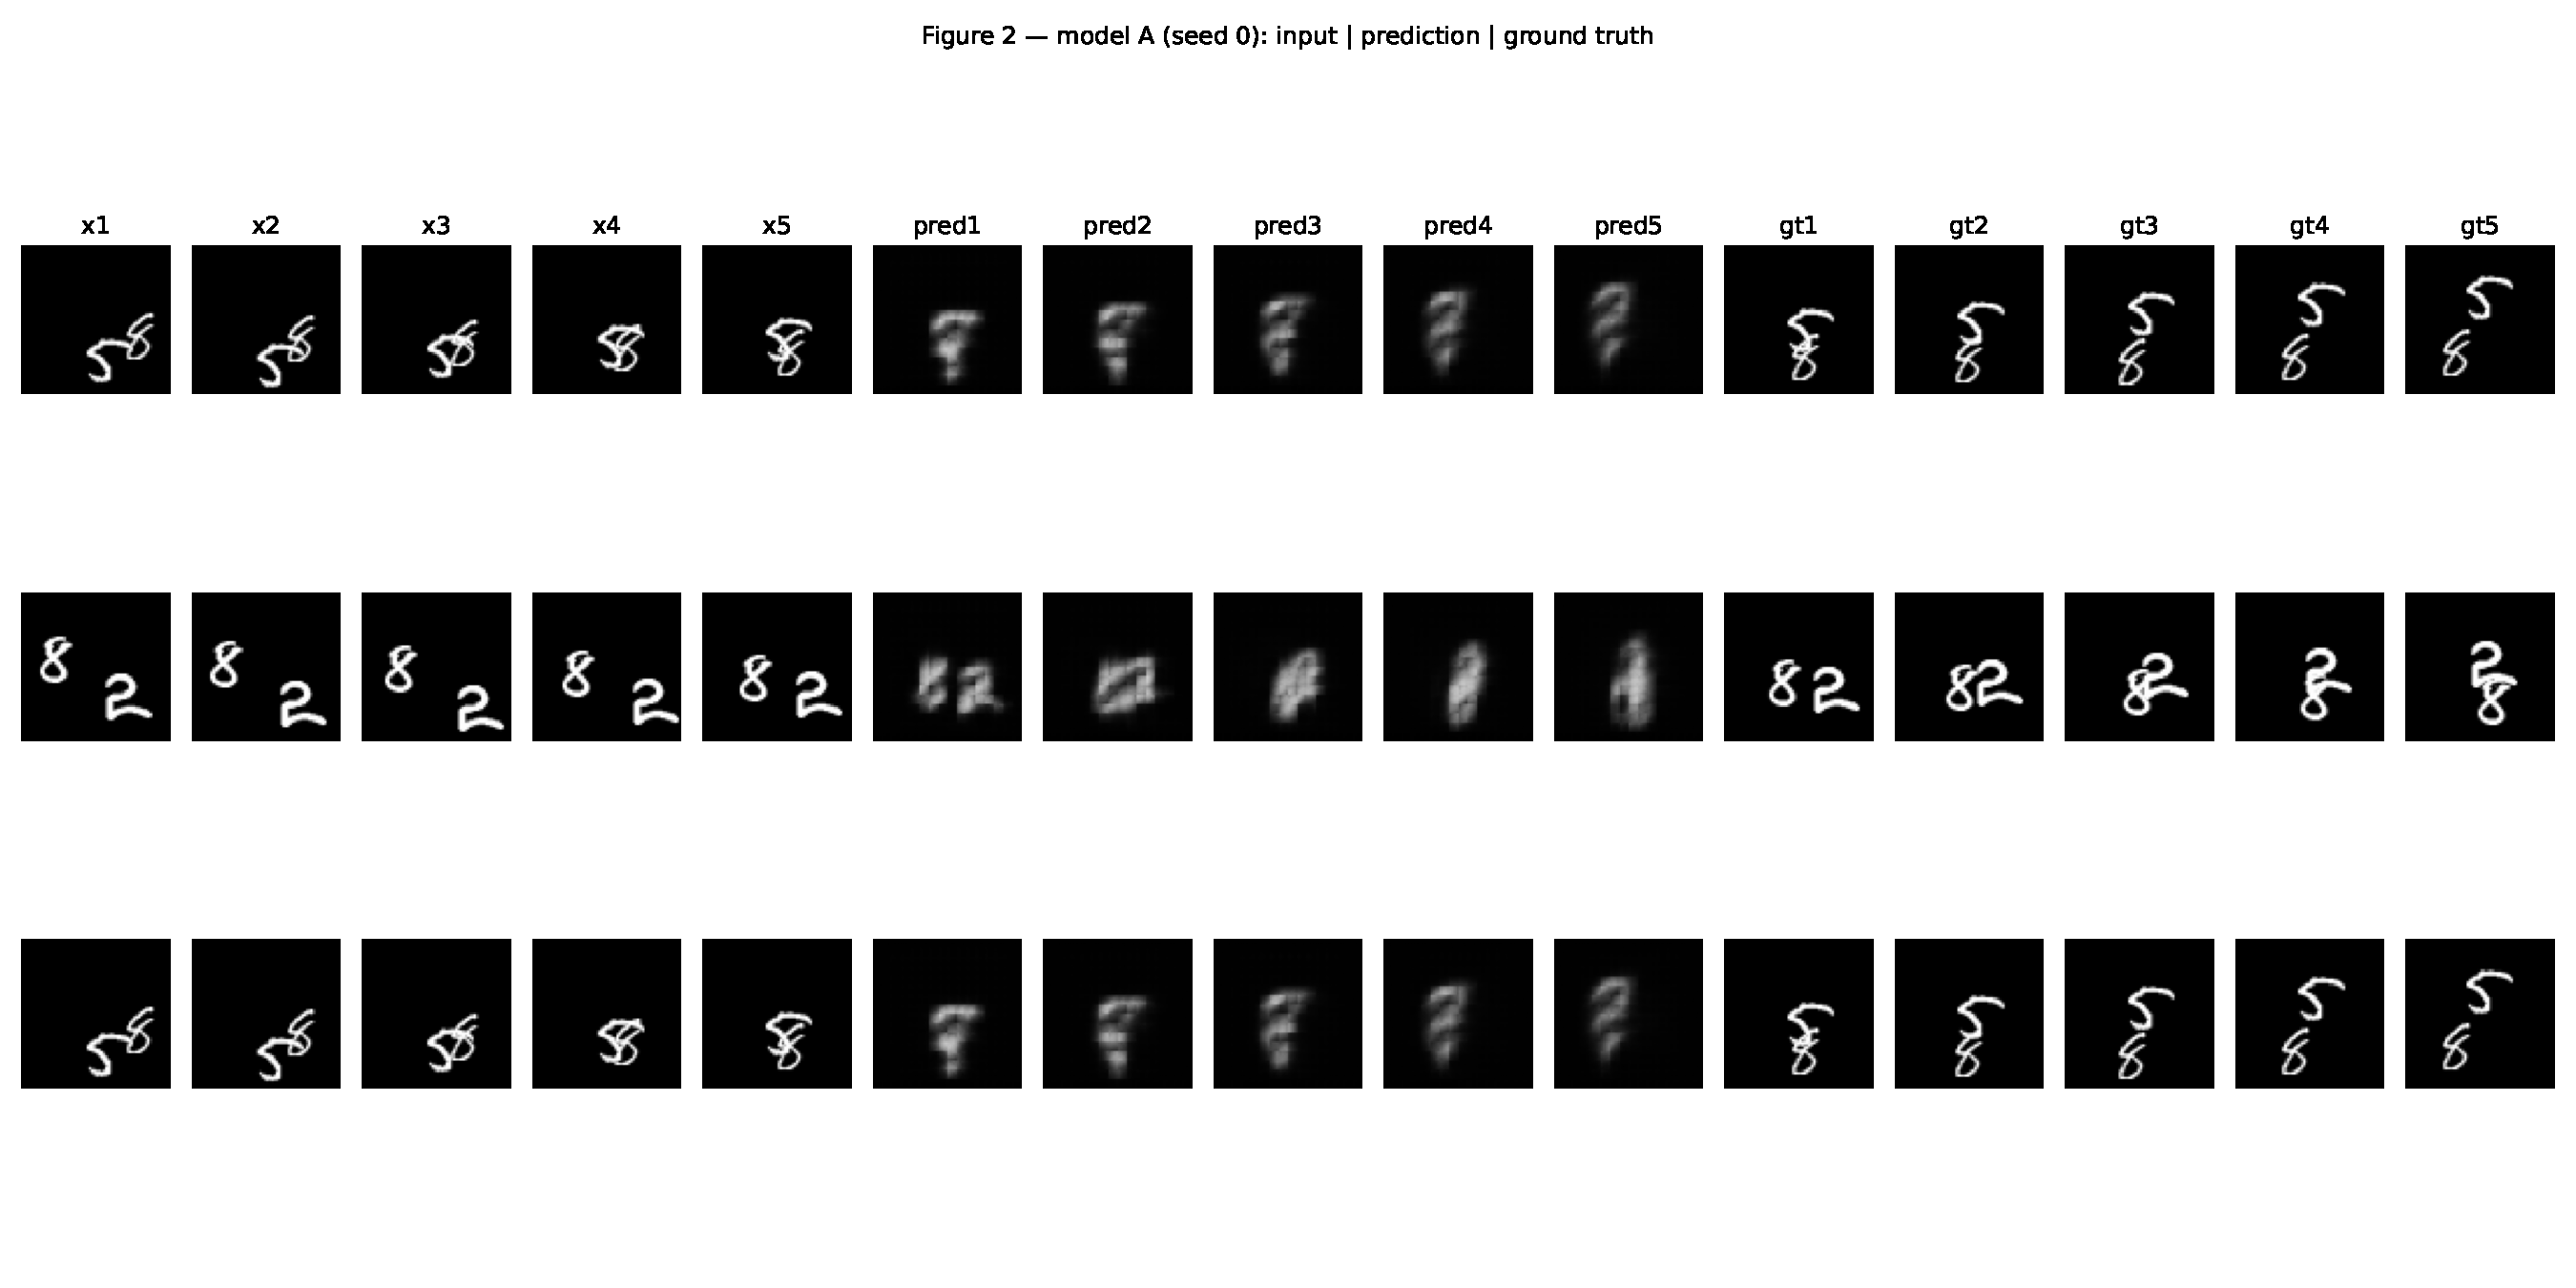
\includegraphics[width=\textwidth]{figure2.pdf}
\caption{Figure 2 --- model A (seed 0): inputs, predictions, ground truth on three test videos (one with overlap).}
\end{figure}

\textbf{Q2.4.} A beats Blank and Copy-last on every horizon. Error grows steadily with $h$ (0.0169 $\to$ 0.0258). On overlaps the prediction smears both digits into a blur rather than keeping two sharp identities.

\subsection*{Q2.5 --- before Testing the Baseline (unedited)}

I am writing this before any mirror, rotation, or speed-up test.

Mirror: I do not think model A will pass. The motion rule is the same after a flip, but the digits look different, and training never asked the net to treat a mirrored 2 like a 2. Expect a non-zero $C_M$ and a clear rise in $E_M$.

Rotation: same story, probably worse. Expect $C_R,E_R$ above the mirror numbers.

Speed: reach $\approx 8$ px/step. If typical motion is only a couple of pixels per frame at 1$\times$, then 2$\times$ may still be close and 3$\times$ is where it should break (blur, stall, or a digit left behind).

\subsection*{Table 3--4, Figures 3--5}

\begin{center}
\small
\begin{tabular}{lccccc}
\toprule
Model & $E(5)$ & $C_M$ & $E_M$ & $C_R$ & $E_R$ \\
\midrule
A & 0.0219 (0.0224, 0.0214) & 0.00176 (0.00175, 0.00177) & 0.0225 (0.0230, 0.0221) & 0.00315 (0.00307, 0.00323) & 0.0237 (0.0241, 0.0233) \\
Blank & 0.0426 & 0 & 0.0426 & 0 & 0.0426 \\
Copy-last & 0.0641 & 0 & 0.0641 & 0 & 0.0641 \\
\bottomrule
\end{tabular}
\end{center}
\noindent
Table 3 --- 1$\times$, $t=1$.

\begin{figure}[H]
\centering
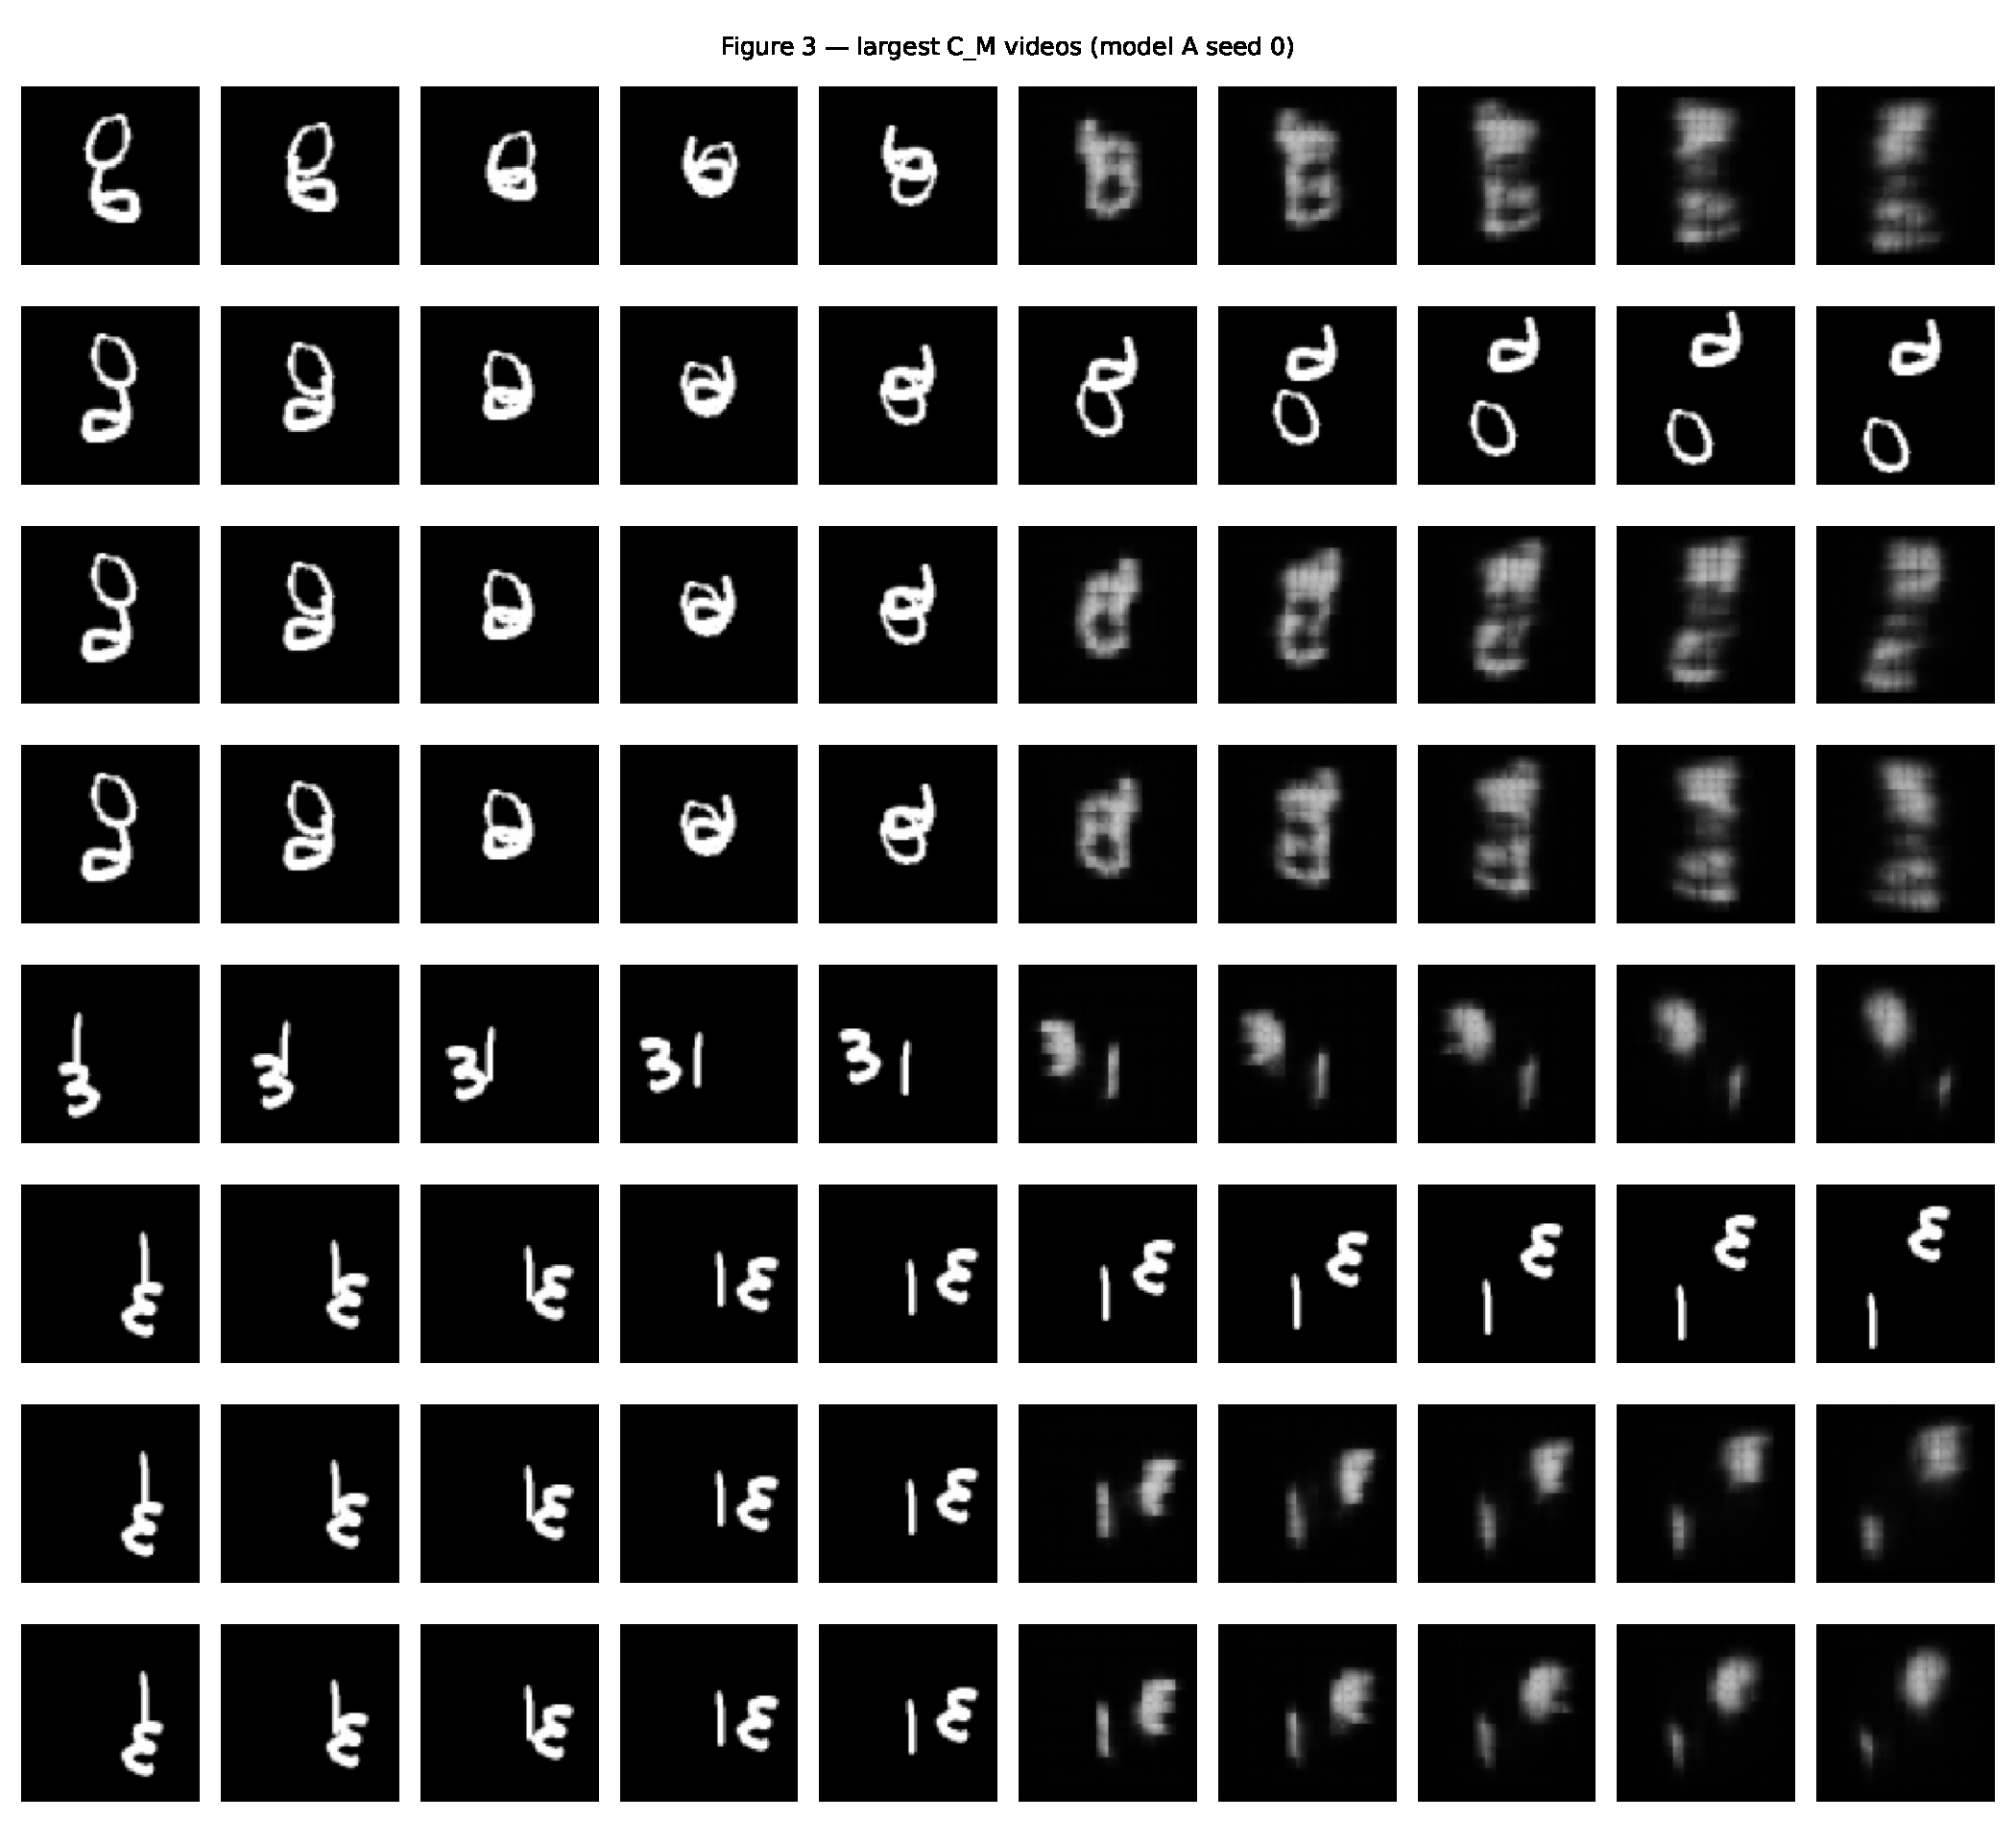
\includegraphics[width=\textwidth]{figure3_M.pdf}\\[0.3em]
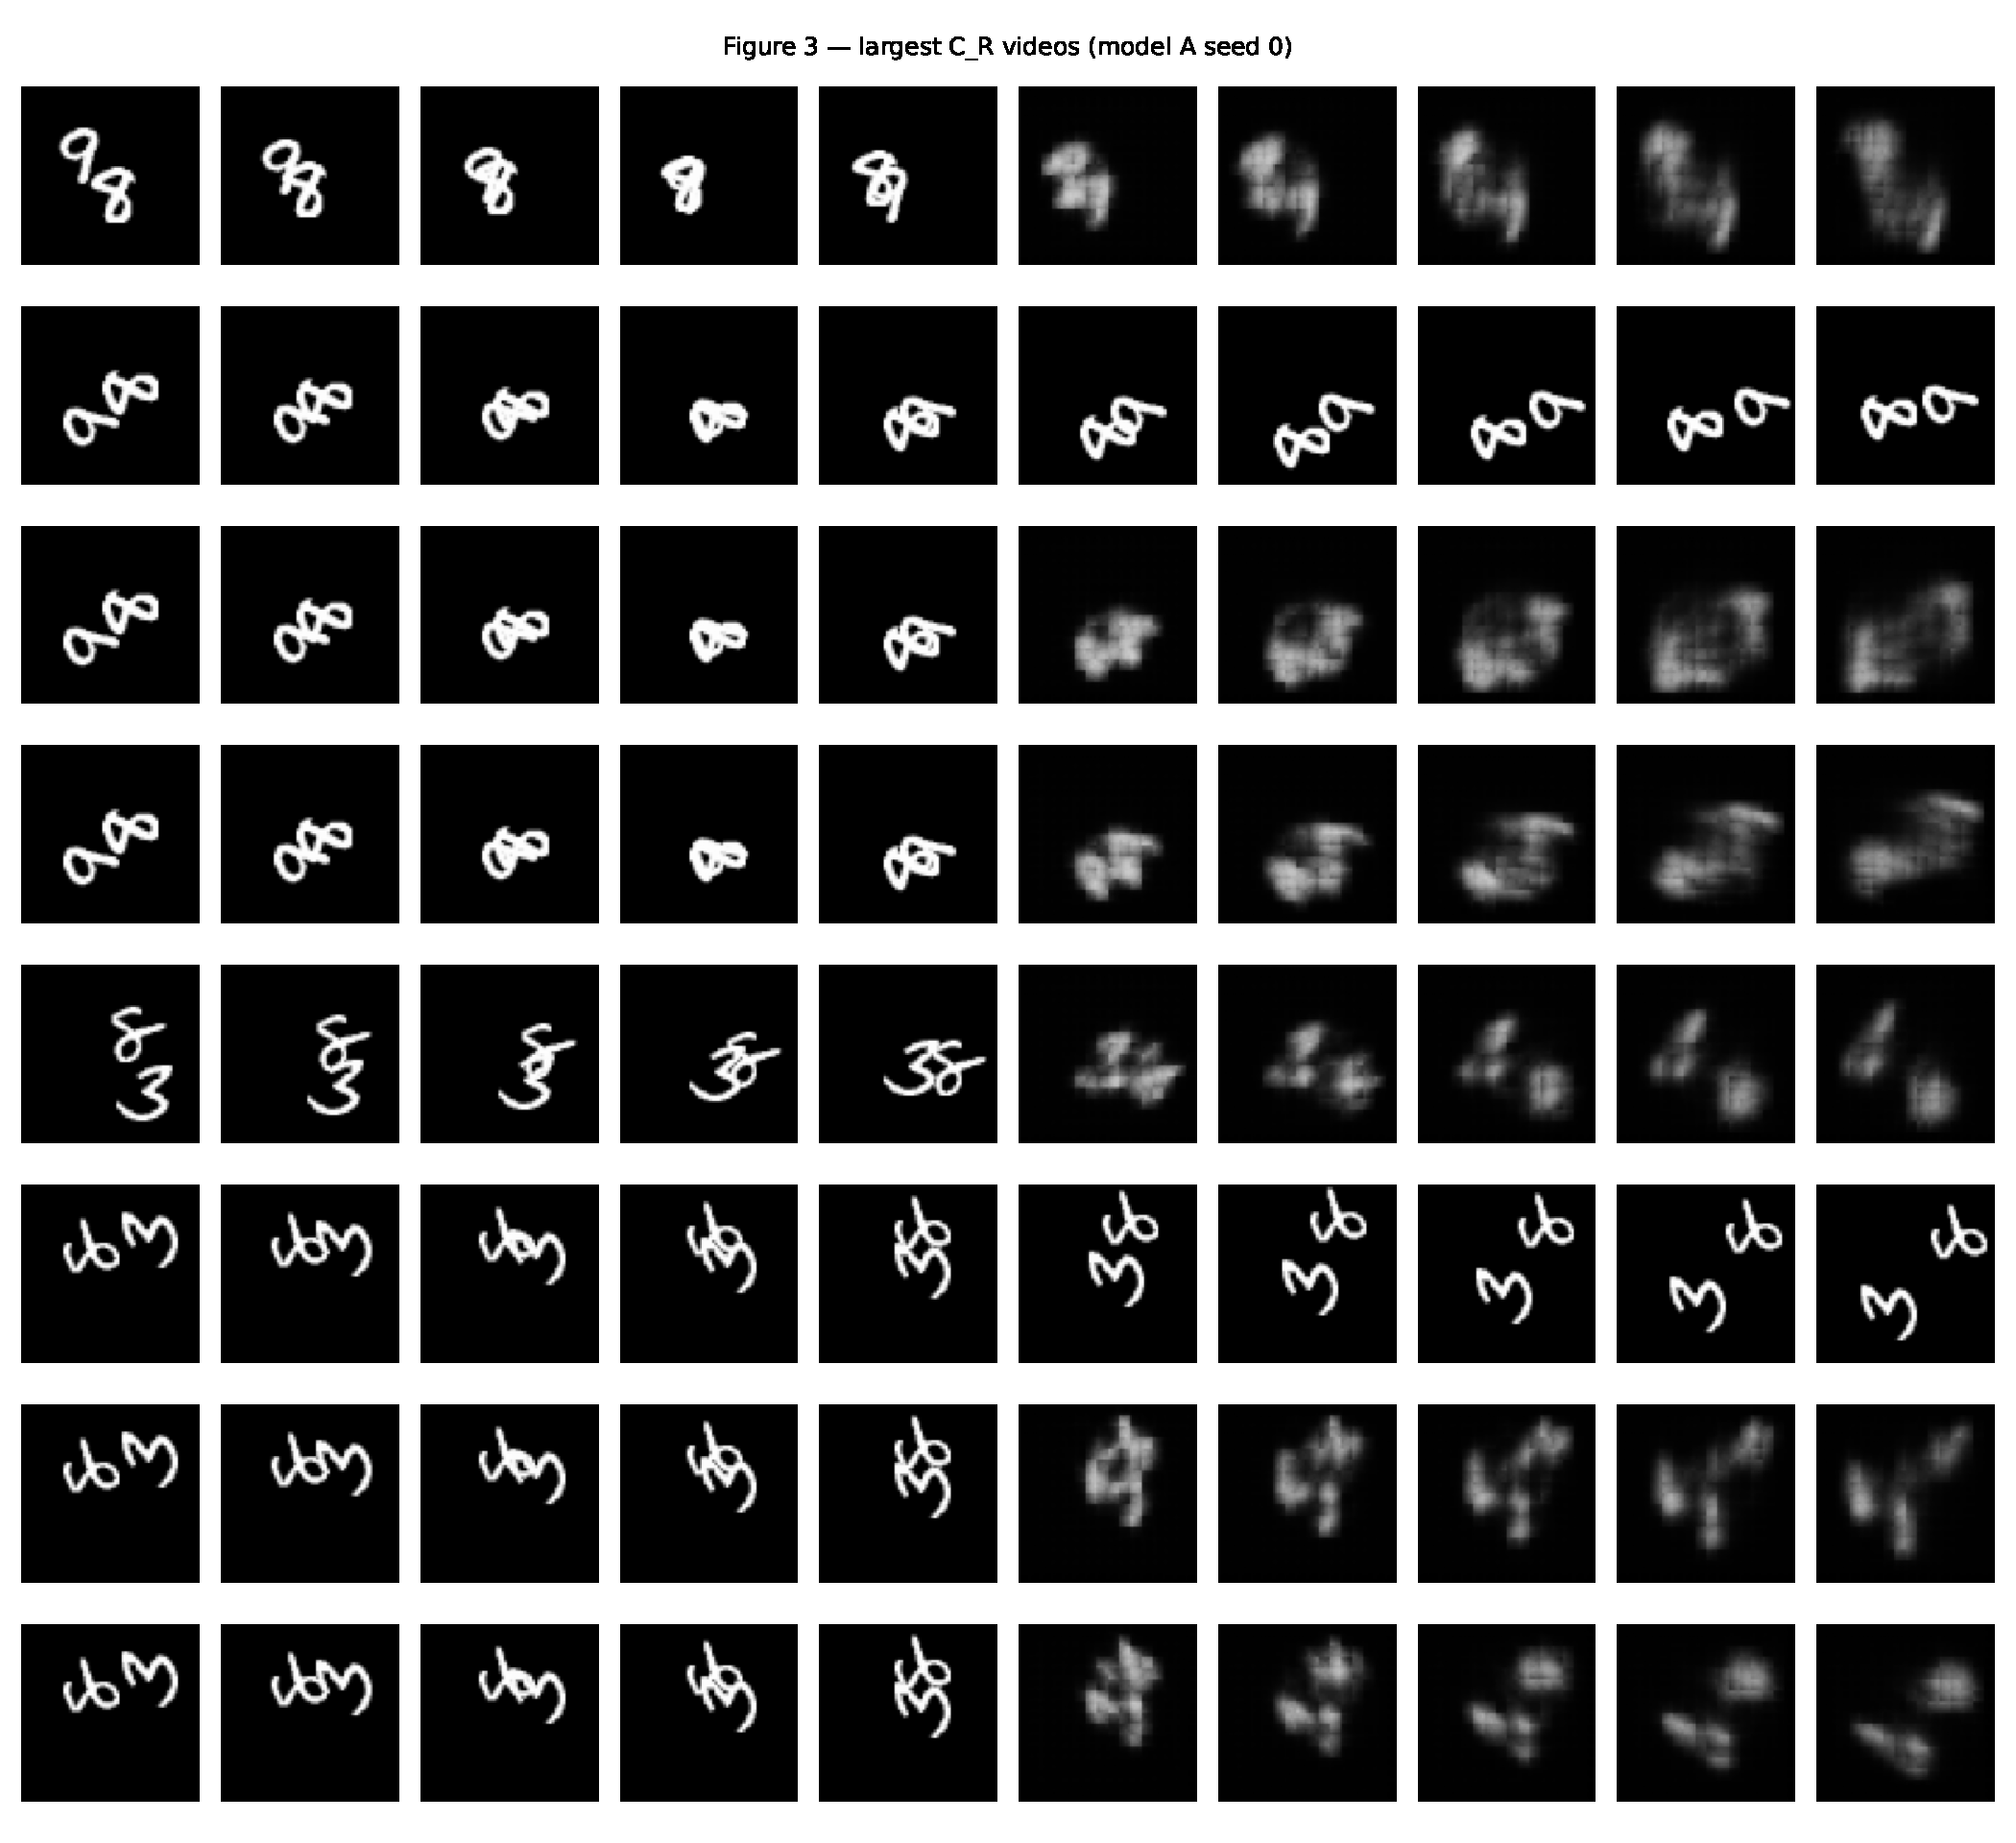
\includegraphics[width=\textwidth]{figure3_R.pdf}
\caption{Figure 3 --- largest per-video $C_M$ (videos 671, 118) and $C_R$ (279, 254), model A seed 0.
GIFs: \texttt{Question2/results/gifs/fig3\_M\_vid671.gif}, \texttt{.../fig3\_M\_vid118.gif}, \texttt{.../fig3\_R\_vid279.gif}, \texttt{.../fig3\_R\_vid254.gif}.}
\end{figure}

\begin{figure}[H]
\centering
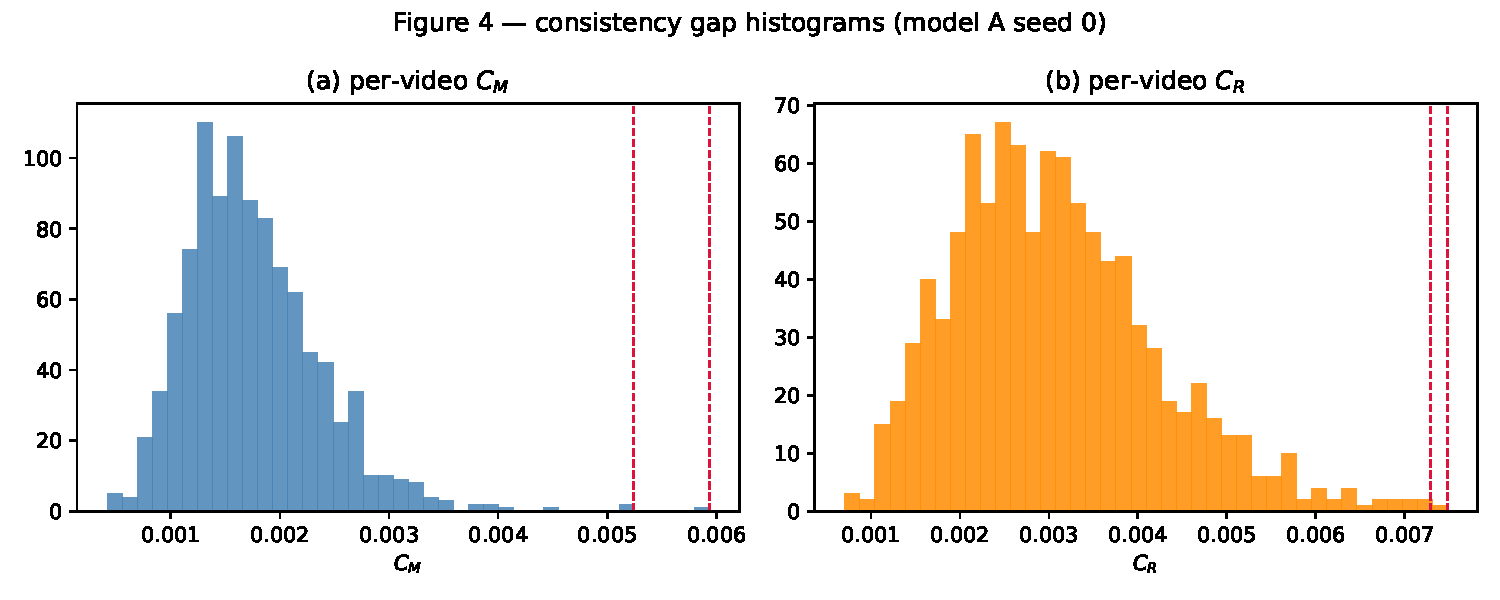
\includegraphics[width=0.95\textwidth]{figure4.pdf}
\caption{Figure 4 --- per-video $C_M$ and $C_R$ histograms (model A seed 0); Figure 3 videos marked.}
\end{figure}

\textbf{Q2.6.} Blank and Copy-last have $C_T=0$ because zeros stay zeros and ``copy last then transform'' equals ``transform then copy last''. Consistency alone is cheap; $E_T$ shows they are still wrong.

\textbf{Q2.7.} On a high-$C_M$ video in Figure 3, rows 3 and 4 disagree: $f(T(X))$ sends a digit the wrong way along the wall while $T(f(X))$ keeps the flipped bounce. The model’s motion account is tied to the digit’s painted shape, not only to the velocity field.

\textbf{Q2.8.} Rotation is a bit harder ($C_R>C_M$, $E_R>E_M$). From Q2.1--Q2.2 that fits appearance more than motion: directions were already somewhat familiar after a $90^\circ$ turn, but digit shapes change more under $R$ than under $M$.

\begin{center}
\small
\begin{tabular}{lccccc}
\toprule
Model & $E(2)$ 1$\times$ & $E(2)$ 2$\times$ & $E(2)$ 3$\times$ & $E(5)$ 1$\times$ & $E(5)$ 2$\times$ \\
\midrule
A & 0.0186 (0.0190, 0.0182) & 0.0441 (0.0435, 0.0448) & 0.0511 (0.0505, 0.0516) & 0.0219 (0.0224, 0.0214) & 0.0485 (0.0476, 0.0495) \\
Copy-last & 0.0548 & 0.0661 & 0.0703 & 0.0641 & 0.0719 \\
\bottomrule
\end{tabular}
\end{center}
\noindent
Table 4.

\begin{figure}[H]
\centering
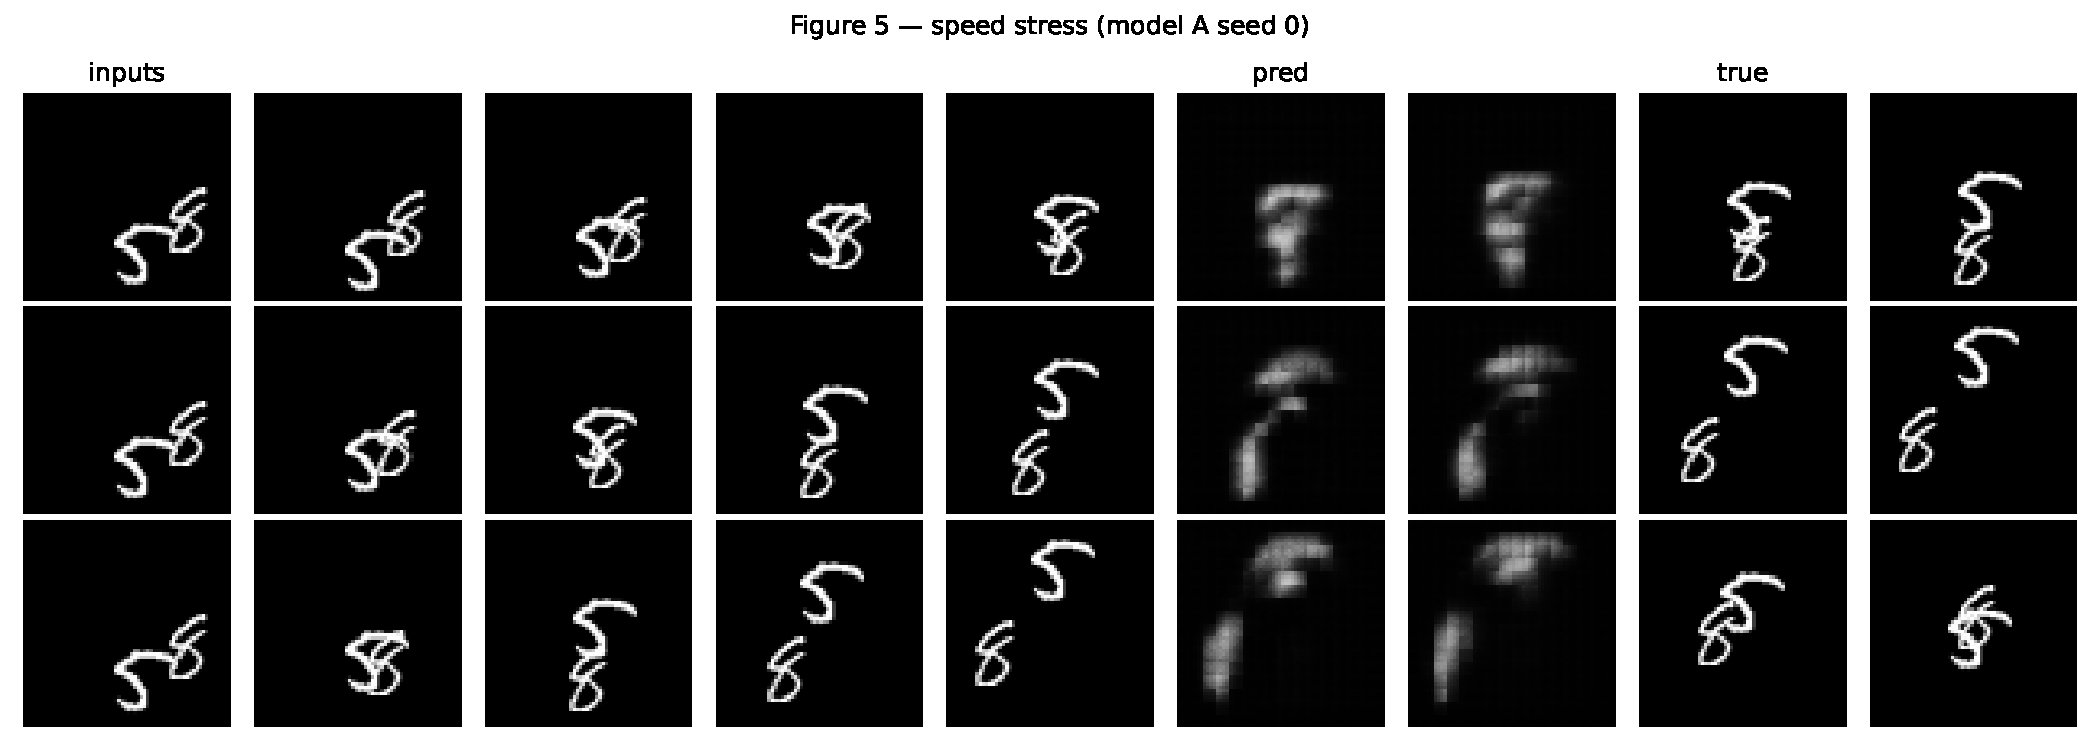
\includegraphics[width=\textwidth]{figure5.pdf}
\caption{Figure 5 --- test video 0 at 1$\times$/2$\times$/3$\times$ (model A seed 0): five inputs, first two predictions, first two true frames.}
\end{figure}

\textbf{Q2.9.} A is fine at 1$\times$, much worse at 2$\times$, and near-useless at 3$\times$ ($E(2)=0.051$). With median speed $3.3$ and reach $8$, 3$\times\approx 9.9$ is past the reach --- agrees with Q2.3. In Figure 5 at 3$\times$ digits blur and stall rather than jump the full gap.

\textbf{Q2.10.} These results alone cannot separate ``never saw fast motion'' from ``beyond reach''. Train the same architecture with speed augmentation (model C) and compare to a larger-reach net also trained with speed aug (model D). If C stays bad at 3$\times$ and D gets better, it was reach.

\subsection*{Q2.11 --- before training B--D (unedited)}

B (symmetry aug) should mainly fix mirror/rotation (appearance). C (speed aug) should help 2$\times$/3$\times$ only up to what reach allows. D (larger reach + speed aug) is the one that should handle 3$\times$ if the speed failure was architectural.

\subsection*{Models B--D and Table 5}

\textbf{Model D:} same 480{,}784 params as A, but ConvLSTM kernels use dilation 2. Reach: radius 2 cells per layer $\times$ 2 layers $=16$ px/step $>8$.

\begin{center}
\scriptsize
\begin{tabular}{lcccccc}
\toprule
 & $E(5)$ 1$\times$ & $C_M$ & $E_M$ & $C_R$ & $E_R$ & $E(2)$ at 1/2/3$\times$ \\
\midrule
A & 0.0219 (0.0224, 0.0214) & 0.00176 & 0.0225 & 0.00315 & 0.0237 & 0.0186 / 0.0441 / 0.0511 \\
B & 0.0221 (0.0223, 0.0220) & 0.00119 & 0.0222 & 0.00160 & 0.0222 & 0.0184 / 0.0439 / 0.0487 \\
C & 0.0268 (0.0265, 0.0271) & 0.00122 & 0.0271 & 0.00244 & 0.0280 & 0.0233 / 0.0287 / 0.0336 \\
D & 0.0283 (0.0281, 0.0285) & 0.00133 & 0.0285 & 0.00221 & 0.0294 & 0.0260 / 0.0289 / 0.0312 \\
\bottomrule
\end{tabular}
\end{center}
\noindent
Table 5 (compressed). Params: A/B/C/D all 480{,}784. Train s/epoch $\approx$ 10.7 / 10.6 / 10.5 / 13.1. Infer s (1000 test, bs 32) $\approx$ 0.73 / 0.73 / 0.73 / 0.89.

\textbf{Q2.12.} D uses dilated $3\times 3$ (dilation 2) in both ConvLSTM layers. Per-layer radius $=2$ folded cells $=8$ px; two layers from the input $\Rightarrow 16$ px/step, strictly above A's 8.

\textbf{Q2.13.} Mirror/rotation: mostly \emph{appearance} --- B cuts $C_M$/$C_R$ while speed is unchanged. Fast motion: partly \emph{unfamiliar motion} --- C drops $E(2)$ at 3$\times$ from 0.051 to 0.034. Residual gap is \emph{architectural reach} --- D gets a bit further (0.031). More 3$\times$ data cannot push information farther than one step’s receptive field; that is why C plateaus above D.

\textbf{Q2.14.} Speed aug costs 1$\times$ accuracy (C/D $E(5)\approx 0.027$ vs A's 0.022). Worth it if the job cares about faster clips; for pure 1$\times$ leaderboard, A/B win.

\subsection*{Final symmetrised model}

$\bar f(X)=\frac18\sum_{g\in G}g^{-1}(f(g(X)))$. Reindexing the finite group average gives $\bar f\circ M=M\circ\bar f$ (same for $R$), so $C_M=C_R=0$ exactly. Final choice: \textbf{symmetrised D} (handout default; Table 5’s 3$\times$ edge for D over C is small but real, and we want exact symmetry).

\begin{center}
\small
\begin{tabular}{lcccccc}
\toprule
Model & $E(5)$ 1$\times$ & $C_M$ & $E_M$ & $C_R$ & $E_R$ & $E(2)$ 3$\times$ \\
\midrule
sym B & 0.0215 (0.0215, 0.0215) & $4.09\times10^{-17}$ & 0.0215 & $1.61\times10^{-17}$ & 0.0215 & 0.0475 \\
sym D & 0.0281 (0.0279, 0.0283) & $3.39\times10^{-17}$ & 0.0281 & $1.34\times10^{-17}$ & 0.0281 & 0.0309 \\
\bottomrule
\end{tabular}
\end{center}
\noindent
Table 6 --- $C_T$ in scientific notation (float noise around 0). Infer $\approx 3.4$\,s (sym B) / $4.6$\,s (sym D). Train time is that of the underlying B or D.

\begin{figure}[H]
\centering
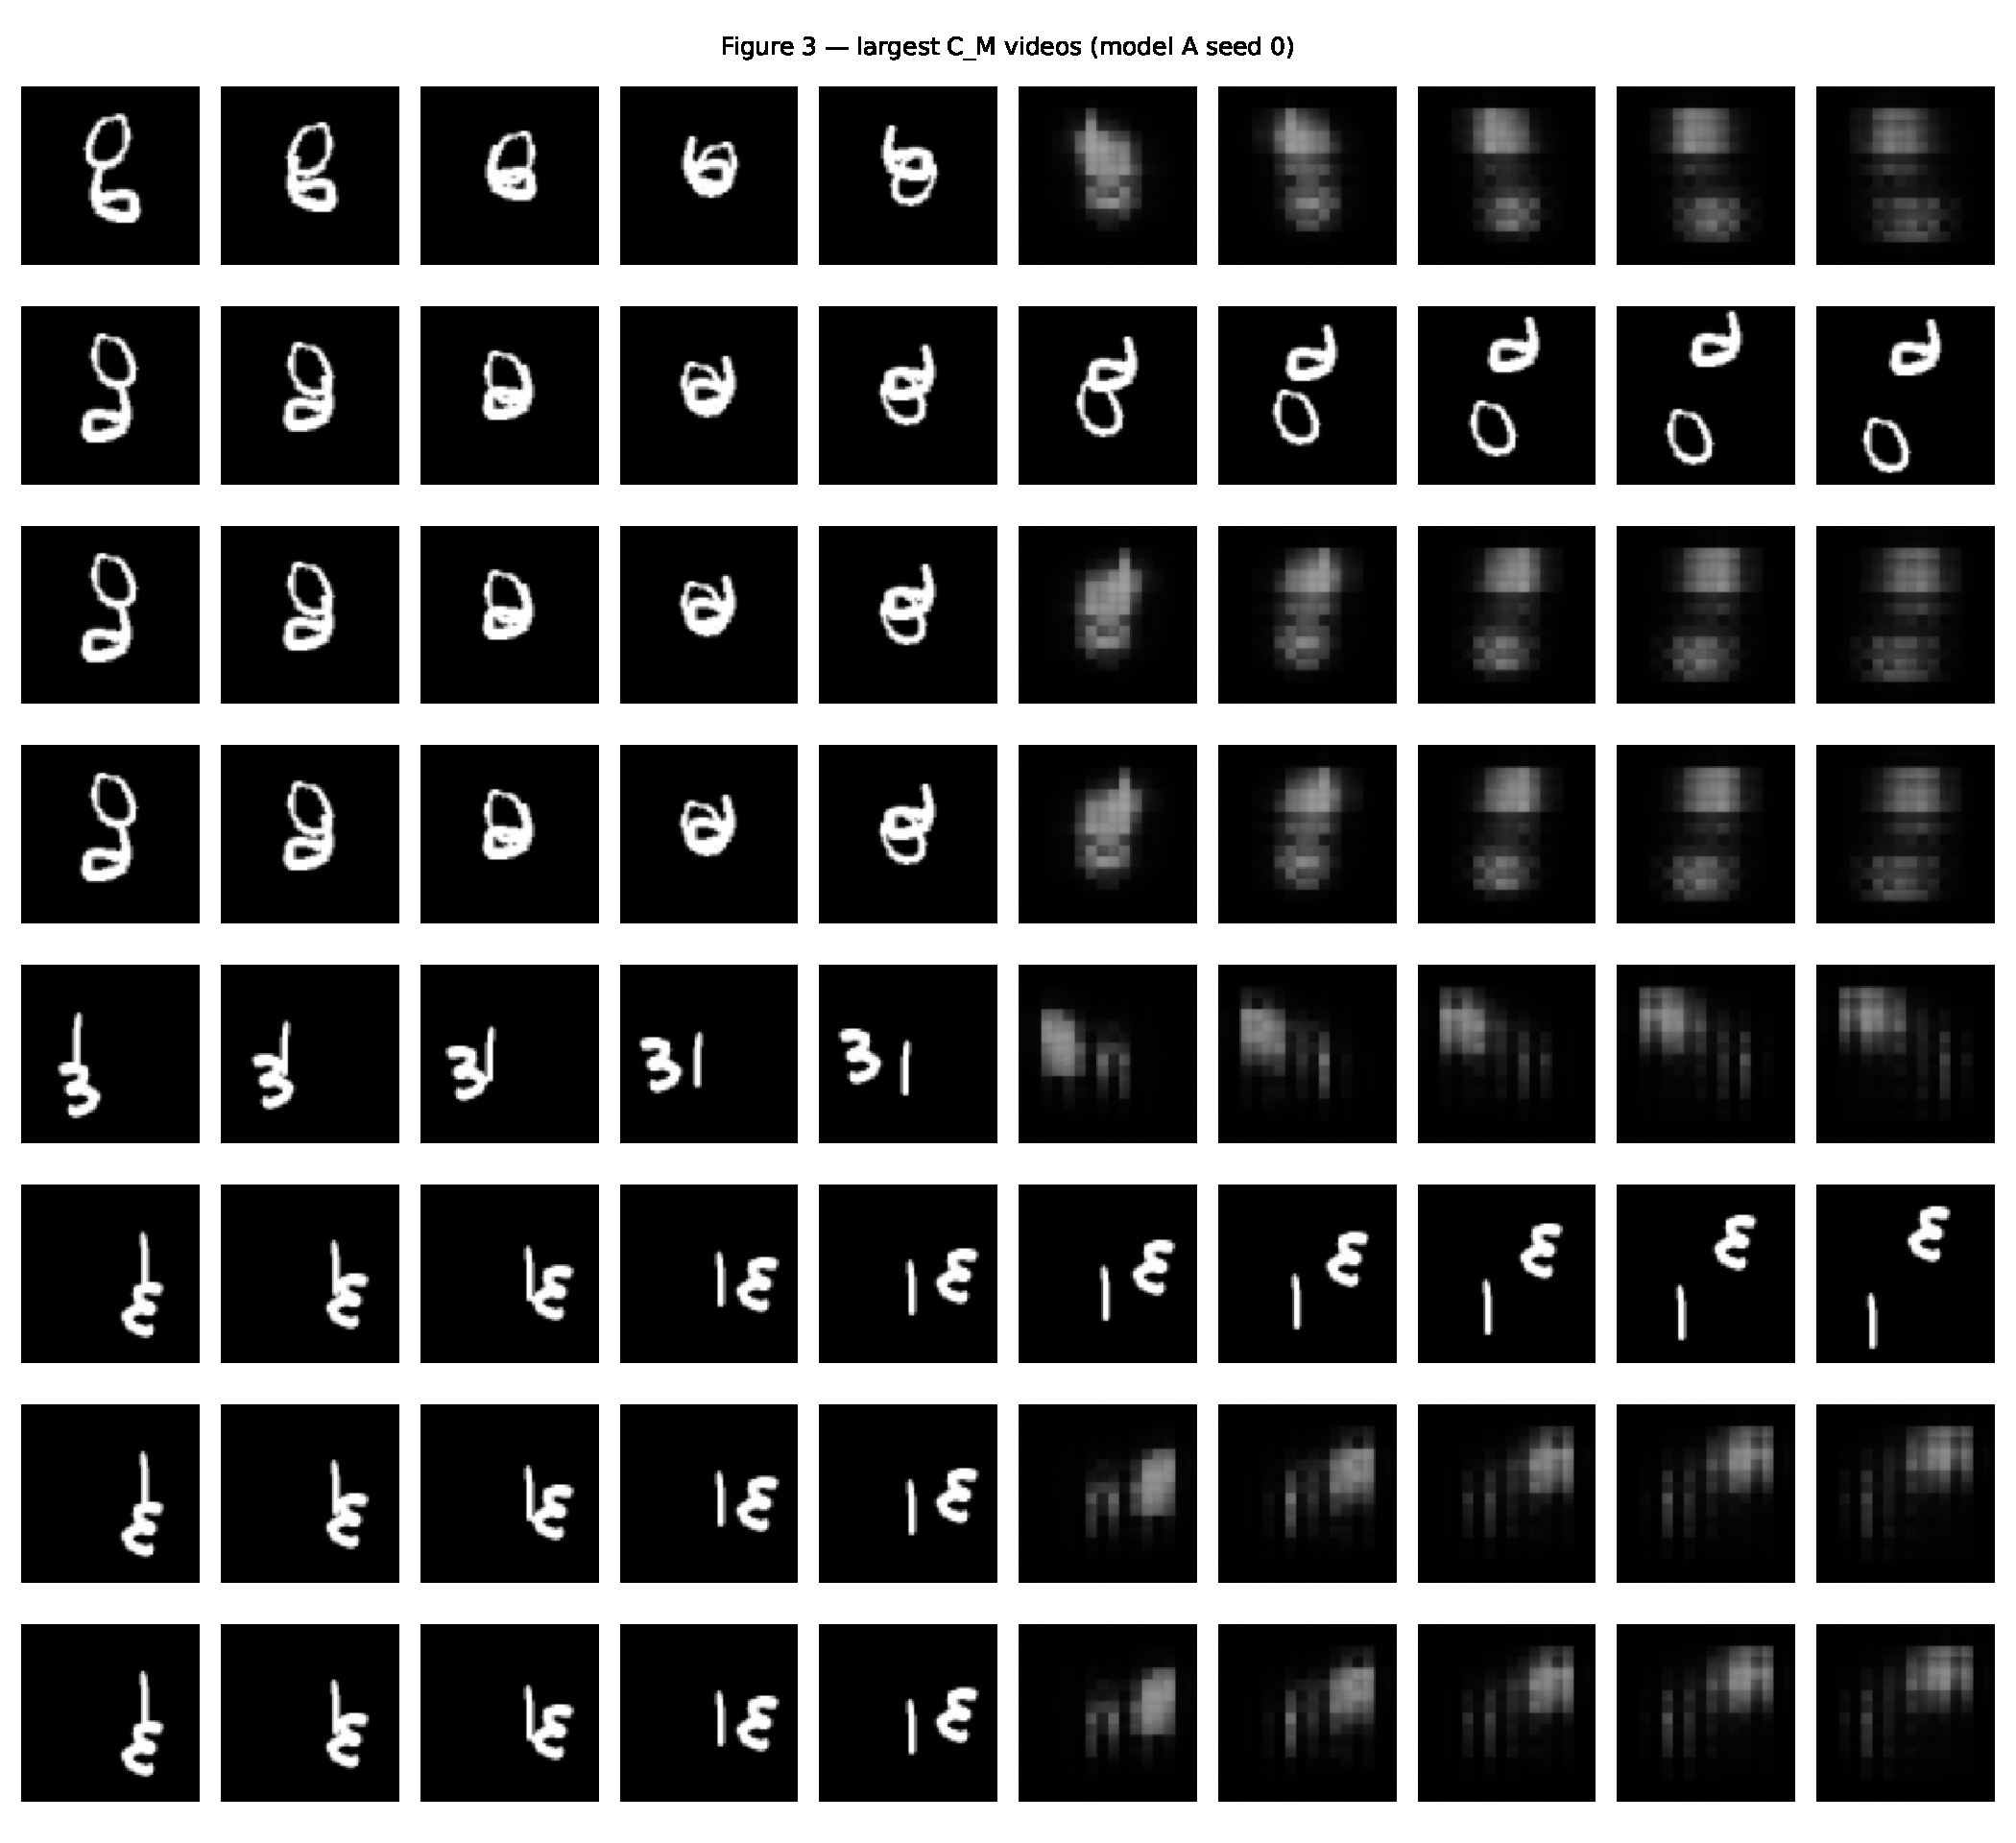
\includegraphics[width=\textwidth]{figure6a_M.pdf}\\[0.2em]
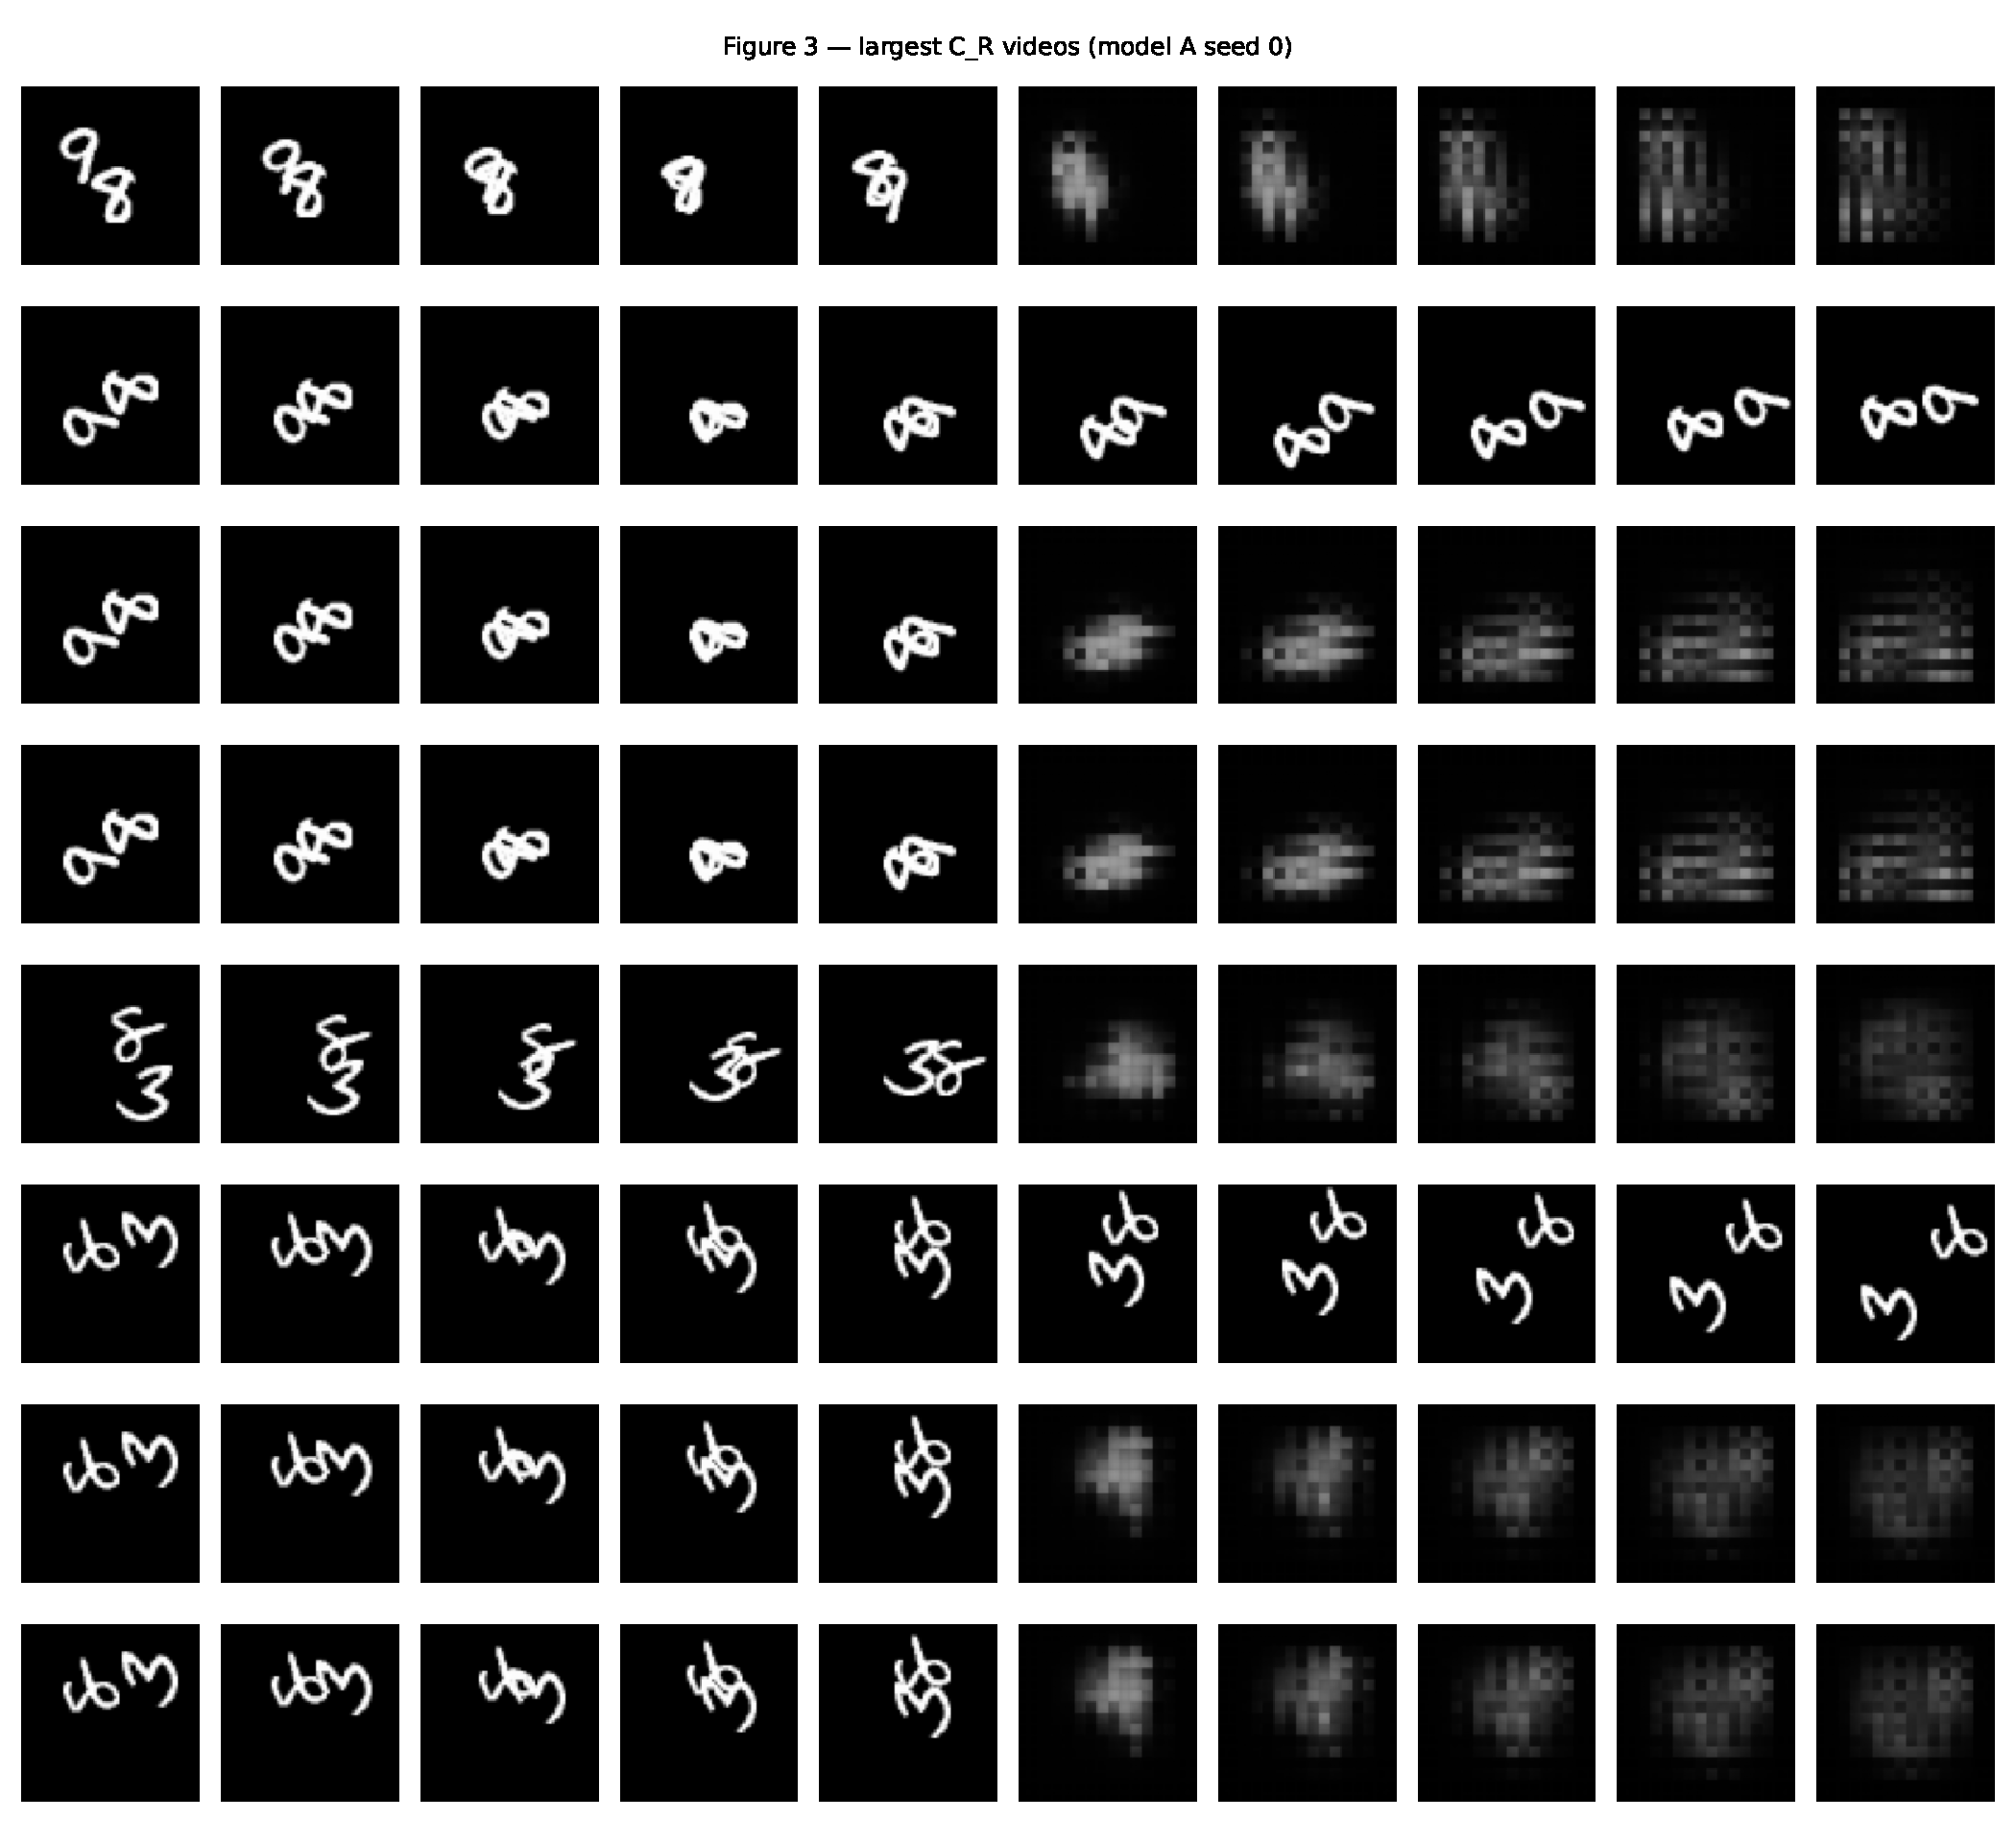
\includegraphics[width=\textwidth]{figure6a_R.pdf}\\[0.2em]
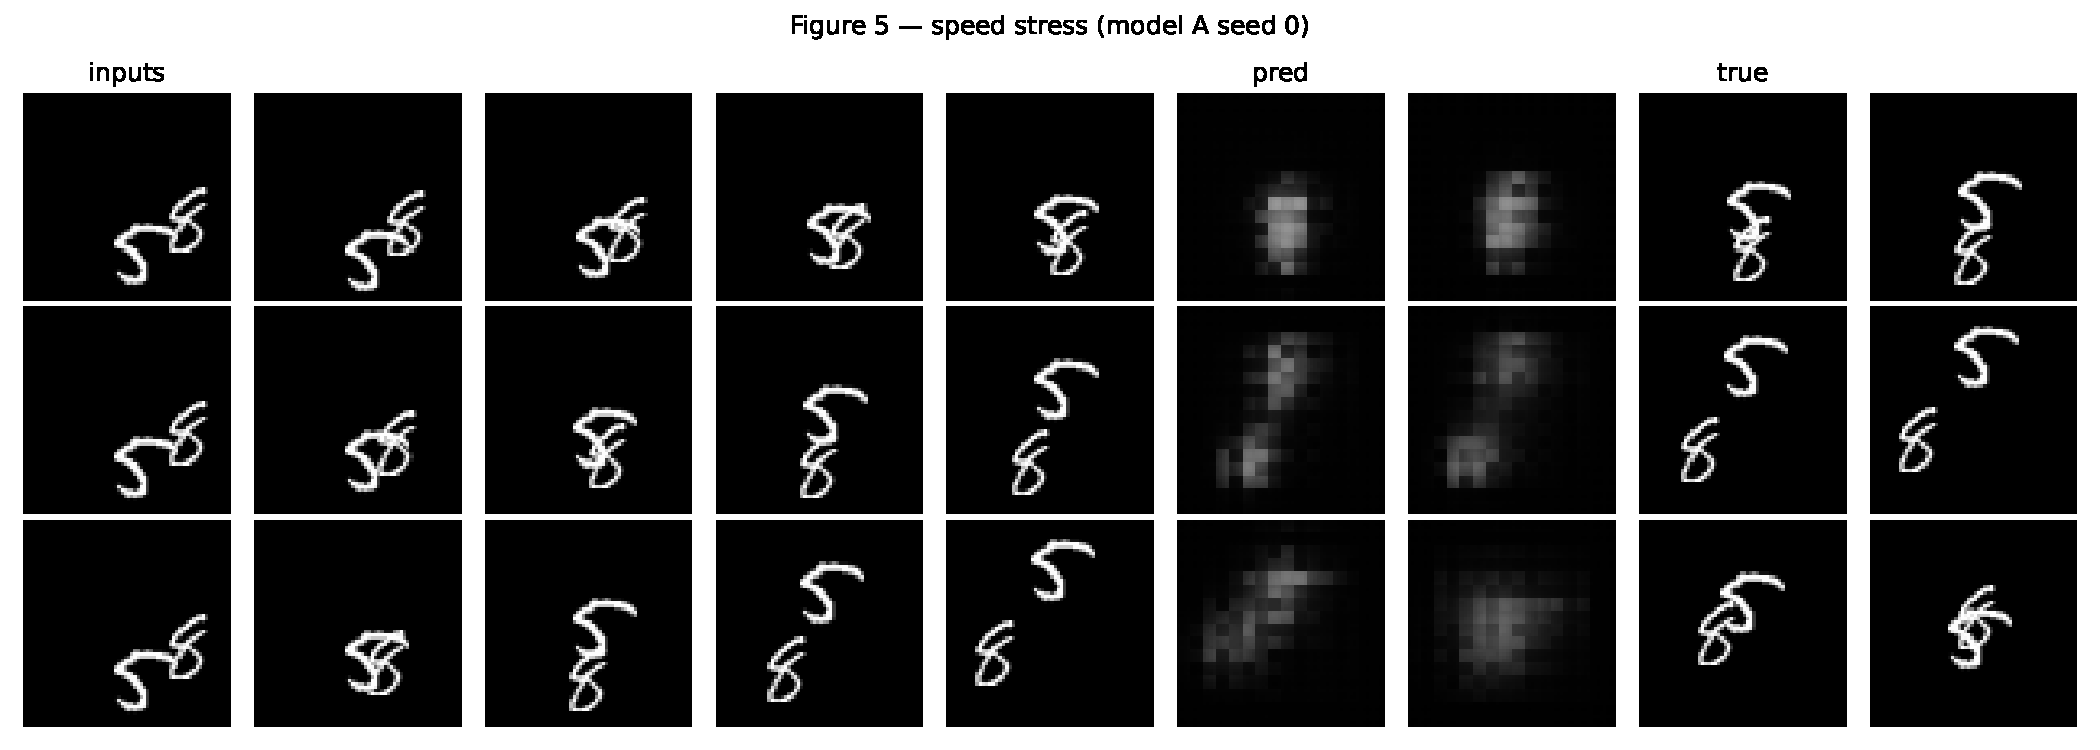
\includegraphics[width=\textwidth]{figure6b.pdf}
\caption{Figure 6 --- (a) Figure 3 videos with final model (sym D); (b) Figure 5 video with sym D.
GIFs under \texttt{Question2/results/gifs\_final/}.}
\end{figure}

\textbf{Q2.15.} Learned symmetry (B) lowers $C_T$ but not to zero. Built-in $\bar f$ is exact ($C_T\sim10^{-17}$) and usually matches or slightly beats $E_T$ of the base model, at $\sim 8\times$ inference cost. Averaging can blur when the eight views disagree; here 1$\times$ error did not get worse for sym B, and sym D kept its 3$\times$ edge.

\textbf{Q2.16.} On the Q2.7 video, sym D’s rows 3 and 4 now match (by construction). The wrong-way bounce from appearance is gone; residual blur at high speed is what speed-aug + reach were meant to fix, and Figure 6b is sharper at 3$\times$ than Figure 5.

\textbf{Q2.17.} Final verdict ($\le$150 words). Symmetrised D does learn motion in the sense that matters here: exact mirror/rotation consistency, and much better 3$\times$ tracking than A. A skeptic should still want a test outside the training speed set --- e.g.\ 4$\times$ or a curved trajectory --- before calling it a general motion engine. One test it has not passed: matching A’s raw 1$\times$ accuracy while staying fast at 3$\times$; the speed-aug tax is still visible.

\section*{AI tools}

Used a chat assistant for ConvLSTM scaffolding and the eval scripts.\\
\textbf{Prompt (rough):} scaffold Moving MNIST ConvLSTM training with mirror/rotation/speed checks for AI651 PA2.\\
\textbf{Got:} folder layout and a first training loop.\\
\textbf{Changed:} Table 1 checks, reach argument, Model D = dilated ConvLSTM, Q2.5/Q2.11 text (committed before those experiments), and the Q1 river design.

\end{document}
